\documentclass[11pt]{article}
\usepackage{float}
\usepackage{graphicx} % Required for inserting images
\usepackage[margin=1in]{geometry}
\usepackage{amsmath,amssymb}
\usepackage{array}
\usepackage{booktabs}
\usepackage{tabularx,tikz,placeins}
\usetikzlibrary{arrows.meta,positioning,fit}
\usepackage{enumitem}
\usepackage{xcolor}
\newcommand{\todo}[1]{%
    \textcolor{red}{\textbf{TODO:} #1}%
}
\usepackage{indentfirst}
\setlength{\parindent}{2em}
\usepackage[super,square,sort&compress]{natbib}
\usepackage{hyperref}
\usepackage{setspace}


\setstretch{1.10}
\setlength{\emergencystretch}{2em}

\hypersetup{
    colorlinks=true,
    linkcolor=blue!50!black,
    urlcolor=blue!50!black,
    citecolor=black
}

% --------------------
% Course information
% --------------------
\newcommand{\course}{DSA4213: Natural Language Processing for Data Science}
\newcommand{\semester}{Semester 1, AY2026/2027}

\begin{document}

\begin{center}
{\LARGE\bfseries Group Project Proposal}\\[0.4em]
{\large Improving Repository Navigation and Bug Localization in Minimal Software Engineering Agents}\\[0.9em]
Group ID: 25\\[0.9em]
\course\\
\semester
\end{center}

% ====================
% Administrative information
% ====================
\section*{Administrative Information}

\begin{tabular}{@{}>{\bfseries\raggedright\arraybackslash}p{0.25\linewidth}
                    >{\raggedright\arraybackslash}p{0.70\linewidth}@{}}
Group members & ZHANG YUHANG(A0351628B) \\ &WANG CHI(A0357310M)  \\ &CHEN WENWEN(A0351705J) \\ &JIANG ZHANGZHANG(A0355183B)\\&CHEN XINGYU(A0355370E) \\[0.7em]

Project direction & Software Engineering Agents -- Repository Navigation and Bug Localization. \\[0.7em]
Repository & \url{https://github.com/235559649/DSA4213_group_work} \\
\end{tabular}

% ====================
% Executive summary
% ====================
\section*{Project Summary}

Software engineering agents such as mini-SWE-agent can autonomously explore repositories, modify code, and execute tests, but repository exploration is largely driven by free-form shell interaction. This project studies whether structured repository navigation and failure-aware bug localization can improve the efficiency and reliability of software repair agents. We will extend mini-SWE-agent with a Python-oriented repository indexer that ranks relevant files and functions based on issue descriptions, code structure, and runtime failure evidence. We will compare the proposed agent with the original mini-SWE-agent on real bug-fixing tasks, evaluating repair success rate, localization accuracy, number of explored files, shell commands, token usage, runtime, and failure patterns.

% ====================
% 1. Problem and motivation
% ====================
\section*{1. Problem, Research Question, and Motivation}

\todo{CHEN WENWEN}

Software engineering agents must often explore a large repository before
they can determine which files or functions are responsible for a reported
bug. A minimal agent such as mini-SWE-agent can perform this exploration
using shell commands and language-model reasoning, but the navigation
process is not explicitly optimized for locating relevant code.

Our project focuses on the repository exploration and bug localization
stage of the software repair process. Rather than replacing the existing
repair capability of mini-SWE-agent, we investigate whether additional
repository structure and runtime failure evidence can help the agent
reach relevant code more efficiently.

\todo{Add a short motivating example showing an issue where the agent
must search through several files before reaching the correct function.}

\subsection*{1.1 Primary Research Question}

\textbf{RQ1.}
Can structured repository navigation and runtime failure evidence help
mini-SWE-agent localize relevant code more efficiently without reducing
bug-fixing success?

\subsection*{1.2 Secondary Research Questions}

\textbf{RQ2.}
Does improved localization reduce repository exploration cost, measured
by the number of files inspected, shell commands executed, token usage,
and runtime?

\vspace{0.5em}

\textbf{RQ3.}
Which information sources contribute most to successful localization:
textual relevance to the issue, static repository structure, or runtime
failure evidence?

\subsection*{1.3 Definition of Success}

The project will be considered successful if the proposed system can
either improve bug localization and repair performance, or achieve
comparable repair performance while reducing unnecessary repository
exploration.

\todo{Define quantitative success criteria after pilot experiments,
for example an improvement in Top-$k$ localization accuracy or a
reduction in exploration steps.}

% ====================
% 2. Related work and contribution
% ====================

\section*{2. Related Work and Proposed Contribution}

\subsection*{2.1 mini-SWE-agent}

Software engineering agents alternate between model decisions, repository operations, and execution feedback. SWE-agent shows that the agent--computer interface (ACI) affects repository-level software repair through the design of commands and feedback \cite{yang2024sweagent}. Building on this insight, we adopt \textbf{mini-SWE-agent} as our baseline: a separate, minimal implementation combining a language model, a command-execution environment, and a linear interaction history \cite{minisweagent}. Its shell interface supports the core operations needed for repair—repository search, code inspection, editing, and test execution. By default, the v2 implementation issues these operations through native bash tool calls, while legacy configurations instead parse commands from model-generated text \cite{minisweagentv2}.

The teal path in Figure~\ref{fig:rw-intervention} shows the agent loop: \emph{decide, act, observe, and update history}. Given the issue and interaction history, the model selects an action, which the environment executes as a shell command. The resulting output, errors, and test results are formatted as observations and appended to the history, alongside the model's response, to inform the next decision \cite{minisweagent}. Across iterations, the agent can locate relevant code, investigate or reproduce a bug, edit files, and run accessible tests. These are available actions rather than a fixed sequence: new evidence may prompt further inspection or another edit. The loop continues until submission or another stopping condition, such as a resource limit. The repository diff provides a candidate patch whose correctness is assessed separately.

Our extension preserves the model adapter, execution environment, and repair loop. It supplies ranked localization context before model decisions and updates that context when execution yields usable failure evidence. The baseline retains ordinary execution feedback, including failures, so the comparison isolates the added value of explicit candidate reranking.

\begin{figure}[htbp]
    \centering
    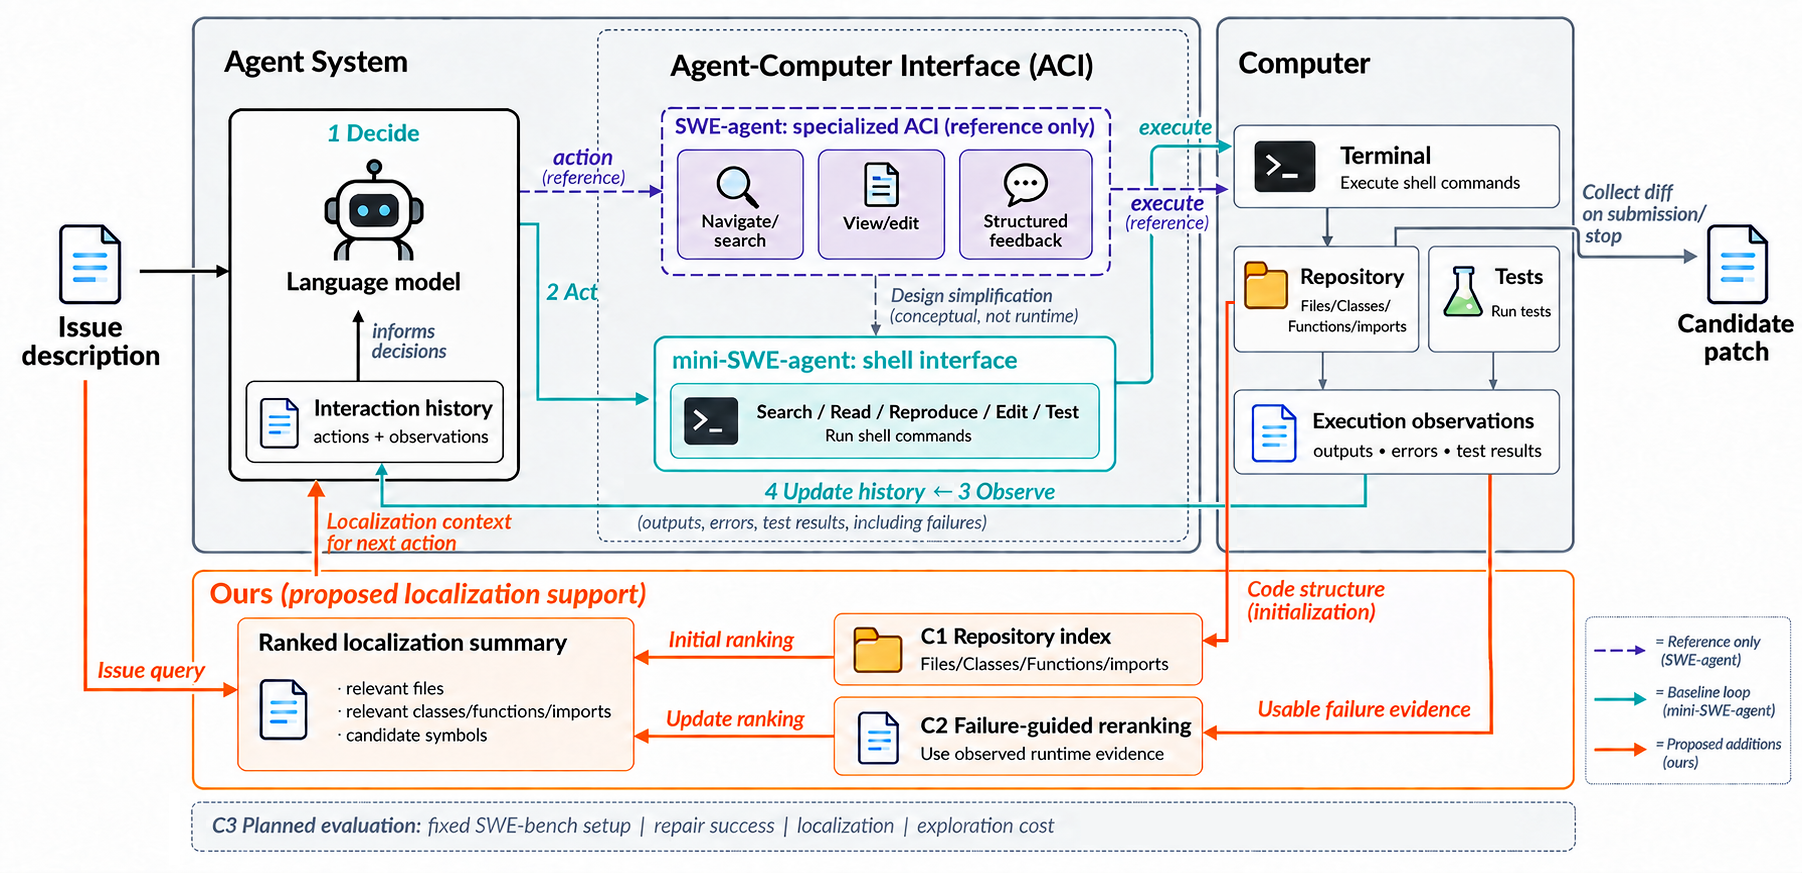
\includegraphics[width=\linewidth]{Fig1 miniSWEagent.png}
    \caption{Overview of mini-SWE-agent and the proposed localization extension.}
    \label{fig:rw-intervention}
\end{figure}


\subsection*{2.2 SWE-bench}

SWE-bench evaluates repository-level software repair using real GitHub issues and executable tests \cite{jimenez2024swebench}. We propose to use \textbf{SWE-bench Verified}, a human-screened subset of 500 tasks from Python repositories \cite{openai2024verified}. Its screening helps reduce ambiguity in issue descriptions and problems with evaluation tests. Its Python scope also matches our repository indexer, making it suitable for examining whether improved localization translates into successful repair.

From this task pool, we initially plan to select approximately 20 tasks for development and 100 additional tasks for evaluation, covering multiple repositories. The development tasks will support debugging and refinement of the localization components. The evaluation tasks will be reserved for comparing the baseline and proposed variants after the method is fixed. We may adjust these target sizes based on runtime and API costs measured during development, before fixing the evaluation task list. The two sets will remain disjoint, and all compared systems will use the same evaluation tasks.


\subsection*{2.3 Repository Localization Methods}

Repository localization uses issue descriptions, code structure,
and execution evidence to identify relevant files and functions.
These information sources support complementary stages of the
search: textual relevance provides initial candidates, structural
relationships guide further inspection, and runtime observations
help revise the search as repair proceeds, as shown in Table~\ref{tab:rw-positioning}.

\begin{table}[H]
\centering
\small
\setlength{\tabcolsep}{3pt}
\renewcommand{\arraystretch}{1.18}
\caption{Prior methods relevant to this study.}
\label{tab:rw-positioning}

\begin{tabularx}{\linewidth}{
    @{}
    >{\raggedright\arraybackslash}p{0.15\linewidth}
    >{\raggedright\arraybackslash}p{0.19\linewidth}
    >{\raggedright\arraybackslash}X
    >{\raggedright\arraybackslash}X
    @{}
}
\toprule
Category & Approach & Relevant mechanism & Role in this study \\
\midrule

Agent framework
& mini-SWE-agent \cite{minisweagent}
& Shell actions and execution feedback in a minimal agent loop.
& Provides the baseline repair loop. \\

\midrule

Textual retrieval
& BugLocator \cite{zhou2012buglocator}
& File ranking using textual similarity and historical bug information.
& Motivates the lexical localization comparison. \\

\midrule

Staged localization
& Agentless \cite{xia2024agentless}
& Hierarchical localization followed by repair and validation.
& Separates candidate selection from patch correctness. \\

\midrule

Structural navigation and reasoning
& LocAgent \cite{chen2025locagent}
& Navigation over code entities and dependency relationships.
& Motivates structural support for code search. \\

& CoSIL \cite{jiang2025cosil}
& Iterative code-graph search with context pruning.
& Motivates refinement of localization context. \\

& RepoNav \cite{chai2026reponav}
& File-centered organization of snippets and candidate functions.
& Motivates structured presentation of candidates. \\

& GraphLocator \cite{liu2025graphlocator}
& Graph-guided reasoning about symptoms and edit locations.
& Distinguishes observed symptoms from repair targets. \\

\midrule

Execution-informed localization
& AutoCodeRover \cite{zhang2024autocoderover}
& Structural search with optional spectrum-based fault localization.
& Connects code structure with test evidence. \\

& IssueExec \cite{liu2026issueexec}
& Test retrieval and execution-trace analysis.
& Links execution evidence to candidate edit locations. \\

\midrule

Proposed integration
& This study (planned)
& Repository indexing and reranking from observed failures.
& Updates localization context within the mini-SWE-agent loop. \\

\bottomrule
\end{tabularx}
\end{table}

\textbf{Textual retrieval and staged localization.}
BugLocator ranks source files using report--code textual similarity
and historical bug information \cite{zhou2012buglocator}.
Agentless organizes issue resolution into localization, repair,
and validation, progressively narrowing the code considered for
modification \cite{xia2024agentless}.
Together, these approaches provide a basis for selecting candidate
locations before generating a patch.
We therefore include a lexical localization condition to examine
how much guidance issue--code matching provides within mini-SWE-agent.
Assessing localization alongside repair will show whether improved
candidate selection translates into successful fixes.

\textbf{Structural navigation and evidence organization.}
LocAgent represents code entities and dependencies in a heterogeneous
graph, allowing the agent to navigate relationships between relevant
locations \cite{chen2025locagent}.
CoSIL combines iterative code-graph search with context pruning
to refine the information considered during localization
\cite{jiang2025cosil}.
RepoNav organizes retrieved snippets around files and candidate
functions, supporting comparison between possible targets within
a file \cite{chai2026reponav}.
These studies show how code relationships and candidate organization
can guide repository exploration beyond textual matching.
They motivate our Python repository index, which records files,
classes, functions, and imports, and supplies a ranked localization
summary for subsequent agent decisions.

\textbf{Execution-informed localization.}
AutoCodeRover combines structure-aware code search with optional
spectrum-based fault localization \cite{zhang2024autocoderover}.
IssueExec retrieves relevant tests and analyzes their execution
traces to identify candidate edit locations \cite{liu2026issueexec}.
These methods establish execution as a source of evidence linking
an issue to the code involved in its behavior.
GraphLocator further motivates examining the relationship between
observed symptoms and locations requiring modification
\cite{liu2025graphlocator}.
Building on this rationale, our proposed component maps tracebacks,
failing-test identifiers, and error messages observed during repair
to indexed code entities.
It then updates the candidate rankings and supplies the revised
summary to the agent before its next decision.

\textbf{Positioning of this study.}
The proposed system combines initial localization from repository
structure with ranking updates from the agent's own execution
trajectory.
Its focus is the connection between observed failures, indexed
code entities, and the localization context used in subsequent
decisions.
The original mini-SWE-agent provides the repair loop and ordinary
execution feedback; our extension adds an explicit ranking update
mechanism.
This design supports a controlled study of how structured
localization context affects repair success and exploration cost.
Table~\ref{tab:rw-positioning} summarizes the relevant mechanisms
and the design choices they motivate.


\subsection*{2.4 Our Contribution}

Prior work already supports structural navigation and execution-informed localization. Our contribution is a focused extension and controlled study within mini-SWE-agent, asking whether these signals improve localization efficiency without reducing repair success. We retain the three contributions defined in the group proposal:

\begin{itemize}
    \item \textbf{C1: Repository indexing.} A Python-oriented index of files, classes, and functions that supports localization from the issue description.
    \item \textbf{C2: Failure-aware refinement.} A mechanism that maps observed runtime failures to code entities and updates suspicious-location rankings.
    \item \textbf{C3: Empirical evaluation.} A comparison with the original mini-SWE-agent of repair performance and repository exploration efficiency.
\end{itemize}


% ====================
% 3. Agent setup
% ====================
\section*{3. Agent and Task Setup}

This section defines the common task environment used by the original
mini-SWE-agent baseline and our localization-augmented variants. The
software repair setting is kept unchanged across experimental conditions,
while only the localization information supplied to the agent is varied.
This controlled setup allows us to study whether structured repository
information and runtime failure evidence improve repository navigation,
bug localization, and repair efficiency.


% --------------------
% 3.1 Task
% --------------------
\subsection*{3.1 Task}

Each task consists of a natural-language software issue together with the
corresponding version of a Python repository. The agent must inspect the
repository, identify source code relevant to the reported problem, modify
the code, and produce a patch that resolves the issue without introducing
regressions.

The task follows the repository-level software repair setting used by
SWE-bench \cite{jimenez2024swebench}. For each task, the agent is given:

\begin{itemize}[leftmargin=*, itemsep=0.25em]
    \item the natural-language issue description;
    \item the corresponding repository checkout;
    \item access to the repository through the execution environment; and
    \item test or execution feedback generated through the agent's own actions.
\end{itemize}

The agent is not given the reference patch, benchmark evaluation labels,
or ground-truth localization information. These are reserved exclusively
for offline evaluation.

The primary output of each run is a final repository patch. In addition,
we record the observable agent trajectory, including model responses,
selected actions, shell commands, inspected files, localization rankings,
code edits, test outputs, token usage, and runtime information. These
trajectories will support the localization and exploration-efficiency
analyses described in Section~5.


% --------------------
% 3.2 Operating Environment
% --------------------
\subsection*{3.2 Operating Environment}

The agent will operate in an isolated execution environment compatible
with the SWE-bench evaluation infrastructure. Each task environment
contains the corresponding repository version together with its required
dependencies and available testing infrastructure.

Within the environment, the agent can perform normal software engineering
operations, including:

\begin{itemize}[leftmargin=*, itemsep=0.25em]
    \item navigating the repository using shell commands;
    \item reading and searching source files;
    \item executing Python programs and project-specific commands;
    \item modifying source files;
    \item inspecting Git diffs; and
    \item running available tests or reproduction scripts.
\end{itemize}

The official SWE-bench evaluation harness will be used only for the final
assessment of the submitted patch. Tests executed by the agent during its
trajectory provide intermediate feedback but do not replace the benchmark's
official evaluation.

For reproducibility, we plan to use the task-specific containerized
environments provided by the SWE-bench infrastructure. Different
repositories may require different Python and dependency versions, so
each task will retain its benchmark-specified environment rather than
being forced into a single Python version.

All experimental conditions will use the same repository versions,
execution environments, and resource constraints. The final SWE-bench
release, container configuration, and mini-SWE-agent version will be
pinned before held-out evaluation.


% --------------------
% 3.3 Agent and Experimental Conditions
% --------------------
\subsection*{3.3 Agent and Experimental Conditions}

mini-SWE-agent provides the common software repair agent and interaction
loop for all experimental conditions \cite{minisweagent}. At each step,
the language model receives the issue description and current interaction
history, selects an action, executes that action in the repository
environment, observes the result, and uses the updated history to decide
its next action.

Our system does not replace this repair loop. Instead, it augments the
context available to mini-SWE-agent with explicit localization
information. This design keeps the underlying repair agent fixed while
allowing us to study the contribution of different localization signals.

The study will consider four main experimental conditions:

\begin{itemize}[leftmargin=*, itemsep=0.45em]

    \item[\textbf{A.}]
    \textbf{Original mini-SWE-agent.}
    The agent explores the repository using its standard shell-based
    workflow without additional localization guidance.

    \item[\textbf{B.}]
    \textbf{Lexical localization.}
    The agent receives an initial ranking of repository locations based
    on textual relevance between the issue description and indexed
    source-code entities.

    \item[\textbf{C.}]
    \textbf{Structure-aware localization.}
    The agent receives localization context that combines lexical
    relevance with structural information extracted from the
    Python repository index.

    \item[\textbf{D.}]
    \textbf{Structure-aware localization with failure-aware refinement.}
    The agent begins with the localization information used in
    Condition C and receives an updated ranking when usable runtime
    failure evidence becomes available.

\end{itemize}

A single fixed language model will be used across Conditions A--D so that
performance differences cannot be attributed to different model
capabilities. The same mini-SWE-agent version, base prompt, execution
environment, resource limits, and generation settings will be used in all
conditions.


For the planned experiments, we will use
\texttt{openai/gpt-5.4-mini} as the underlying language model for all
experimental conditions. mini-SWE-agent supports this model through its
LiteLLM-based model interface.

The same model version, reasoning-effort setting, base prompt, generation
configuration, and resource limits will be fixed across Conditions A--D.
Therefore, the prescribed localization information will be the primary
systematic difference between the experimental conditions.


% --------------------
% 3.4 Localization Information and Agent Tools
% --------------------
\subsection*{3.4 Localization Information and Agent Tools}

The original mini-SWE-agent retains its normal shell-based interaction
with the repository. Our extension adds a localization layer that provides
structured guidance rather than restricting the agent to a predefined set
of files.

Before the repair trajectory begins, the repository indexer analyzes the
Python source tree and records code entities including:

\begin{itemize}[leftmargin=*, itemsep=0.25em]
    \item repository-relative file paths;
    \item classes;
    \item functions and methods;
    \item import relationships; and
    \item selected textual and structural metadata used for localization.
\end{itemize}

Given the issue description, the localization module generates a ranked
list of candidate files and code entities. For the initial implementation,
we plan to provide the agent with the top five ranked files. For each file,
up to two highly ranked functions or methods will be included when
function-level candidates are available.

Each localization entry may contain:

\begin{itemize}[leftmargin=*, itemsep=0.25em]
    \item the repository-relative file path;
    \item the class, function, or method name;
    \item the candidate type;
    \item its relevance score or rank; and
    \item a short description of the evidence supporting the ranking.
\end{itemize}

For example, the localization context supplied to the agent may have the
following form:

\begin{verbatim}
1. src/parser.py
   function: parse_header
   score: 0.87
   evidence: strong issue-text match + structural relevance

2. src/io/reader.py
   function: read_table
   score: 0.71
   evidence: related import + lexical relevance
\end{verbatim}

The agent remains free to inspect other repository locations using its
standard shell tools. Therefore, localization acts as navigation guidance
rather than as a hard search constraint.


\subsubsection*{Lexical Localization}

For Condition B, lexical localization will use a BM25-style retrieval
method. Each indexed code entity will be represented using information
such as its file path, identifier, class or function name, docstring, and
selected source text. The issue description will serve as the retrieval
query.

The resulting lexical ranking provides a simple retrieval baseline for
measuring whether explicit issue-to-code matching alone improves
mini-SWE-agent's repository exploration.


\subsubsection*{Structure-Aware Localization}

For Condition C, lexical evidence will be supplemented with repository
structure. The initial structural representation will include containment
relationships between files, classes, and functions, together with import
relationships between Python modules.

Because lexical and structural signals may produce scores on different
numerical scales, we plan to combine their rankings using reciprocal rank
fusion (RRF):

\[
\operatorname{RRF}(x)
=
\sum_{r \in R}
\frac{1}{k + r(x)},
\]

where $r(x)$ is the position of candidate $x$ in one input ranking and
$R$ is the set of rankings being combined. We provisionally set
$k=60$, which will remain fixed unless development-set experiments reveal
a clear implementation problem.

This approach allows different evidence sources to contribute to the final
candidate ordering without requiring their raw scores to be directly
comparable.


\subsubsection*{Failure-Aware Localization}

For Condition D, runtime failures provide an additional ranking signal.
When a command, reproduction attempt, or test produces a usable failure,
the system extracts available evidence such as:

\begin{itemize}[leftmargin=*, itemsep=0.25em]
    \item exception type;
    \item traceback frames;
    \item repository files appearing in the traceback;
    \item class, function, or method names appearing in the traceback;
    \item failing-test identifiers; and
    \item relevant identifiers mentioned in error messages.
\end{itemize}

These observations are mapped back to entities in the repository index.
Candidates appearing directly in repository traceback frames receive the
strongest runtime evidence, while related test and error-message
information provides secondary evidence.

A runtime-based ranking is then fused with the existing lexical and
structural rankings using the same RRF mechanism. This produces an updated
candidate list without discarding evidence derived from the original issue
description.

The revised localization summary is supplied to mini-SWE-agent before a
subsequent repair decision.

The reference patch and benchmark evaluation labels are never used to
construct or update these rankings.


% --------------------
% 3.5 Benchmark and Task Selection
% --------------------
\subsection*{3.5 Benchmark and Task Selection}

The study will use tasks from \textbf{SWE-bench Verified}, a human-screened
subset of repository-level software engineering problems
\cite{openai2024verified}. Its Python repository setting is compatible
with our Python-oriented repository index and provides executable tests
for determining whether a generated patch resolves the corresponding
issue.

We provisionally plan to use approximately 20 tasks as a development set
and up to 100 additional tasks for held-out evaluation.

The development tasks will be used to:

\begin{itemize}[leftmargin=*, itemsep=0.25em]
    \item implement and debug the repository indexer;
    \item validate lexical and structural localization;
    \item develop the failure-aware refinement mechanism;
    \item select practical prompt and interface formats;
    \item estimate token usage, runtime, and API cost; and
    \item verify that the planned resource limits are feasible.
\end{itemize}

The development and held-out sets will remain disjoint. Once the pilot
stage is completed, the held-out task list, model configuration, resource
limits, and comparison protocol will be frozen before the evaluation
results are inspected.

Tasks will be selected across multiple repositories where possible so
that conclusions are not dominated by a single codebase. The same task
instances will be used across all four experimental conditions.

For file-level localization evaluation, only tasks whose reference patch
contains at least one modified Python source file will contribute to the
localization metrics. Tasks that cannot be scored for localization may
still contribute to the overall repair evaluation when applicable.

The exact task identifiers and repository distribution will be published
in the project repository together with the final experimental
configuration to support reproducibility.


% --------------------
% 3.6 Stopping Conditions and Failure Recovery
% --------------------
\subsection*{3.6 Stopping Conditions and Failure Recovery}

Each agent run will operate under a fixed resource budget. For the initial
proposal, we provisionally plan the following limits:

\begin{itemize}[leftmargin=*, itemsep=0.25em]
    \item maximum of 50 agent interaction steps;
    \item maximum wall-clock runtime of 30 minutes per task; and
    \item maximum total model-token budget of approximately 150,000 tokens
          per run.
\end{itemize}

These limits are intended to prevent unusually difficult tasks from
consuming disproportionate resources. Pilot experiments on the development
set may be used to reduce or adjust these limits if necessary. The final
limits will be frozen before held-out evaluation and applied equally to
all experimental conditions.

A run terminates when one of the following conditions is reached:

\begin{itemize}[leftmargin=*, itemsep=0.25em]
    \item the agent submits a final patch;
    \item the maximum number of interaction steps is reached;
    \item the token or API-cost budget is exhausted;
    \item the wall-clock execution limit is exceeded; or
    \item an unrecoverable environment failure prevents further execution.
\end{itemize}

A patch is not considered successful merely because tests executed by the
agent during repair pass. Final repair success is determined separately
using the official SWE-bench evaluation harness, as described in
Section~5.1.

Failed commands and failed tests are treated as observations rather than
immediate termination conditions. In Conditions A--C, this feedback
remains part of the normal mini-SWE-agent interaction history. In
Condition D, usable failures additionally trigger the localization
refinement mechanism.

A runtime failure is considered usable for localization if at least one
piece of evidence can be mapped back to the repository index. This occurs
when:

\begin{itemize}[leftmargin=*, itemsep=0.25em]
    \item a traceback contains a repository source-file path;
    \item a traceback contains an indexed class, function, or method;
    \item a failing test produces a traceback that reaches project source
          code; or
    \item an error message explicitly mentions an indexed source entity.
\end{itemize}

If none of these conditions is satisfied, the failure does not trigger
reranking and the agent continues using its existing localization context.

The failure-aware repair process can therefore be summarized as:

\begin{center}
Initial ranking
$\rightarrow$
Agent exploration
$\rightarrow$
Execution
$\rightarrow$
Failure evidence
$\rightarrow$
Updated ranking
$\rightarrow$
Continued repair
$\rightarrow$
Final patch.
\end{center}

This design ensures that runtime evidence augments the original issue-based
localization rather than replacing it, while allowing the baseline and
proposed systems to operate under the same repair environment and resource
constraints.


% ====================
% 4. System or study design
% ====================
\section*{4. Proposed System or Study Design}

\todo{CHEN XINGYU}

The proposed workflow consists of an initial repository analysis stage,
a localization stage, the existing mini-SWE-agent repair process, and an
optional refinement stage based on runtime failures.

\begin{figure}[htbp]
    \centering
    \fbox{
        \parbox{0.88\linewidth}{
            \centering
            \vspace{1.5em}
            \todo{Insert system architecture diagram:
            Issue $\rightarrow$ Repository Index
            $\rightarrow$ Initial Localization
            $\rightarrow$ mini-SWE-agent
            $\rightarrow$ Test Execution
            $\rightarrow$ Failure-Aware Refinement
            $\rightarrow$ Repair.}
            \vspace{1.5em}
        }
    }
    \caption{Proposed system architecture.}
\end{figure}


\subsection*{4.1 Baseline}

The baseline is the original mini-SWE-agent operating with its standard
repository exploration and repair loop.

\todo{Describe the exact baseline configuration and ensure it uses the
same LLM and execution budget as the proposed system.}


\subsection*{4.2 Repository Indexing}

Before repair begins, the repository indexer analyzes the Python
repository and records structural information such as:

\begin{itemize}[leftmargin=*, itemsep=0.25em]
    \item file paths;
    \item classes;
    \item functions and methods;
    \item import relationships; and
    \item selected code metadata relevant to localization.
\end{itemize}

\todo{Define the actual internal representation. Decide whether this
will be a table, graph, JSON index, or another structure.}

\todo{Decide whether call relationships or inheritance information are
included. Avoid adding them unless they are actually used.}


\subsection*{4.3 Initial Localization}

Given an issue description, the localization module ranks repository
files and functions according to their estimated relevance to the issue.

The result will be a ranked list of suspicious locations that can be
provided to the repair agent as additional context.

\todo{Define the localization scoring function.}

\todo{Decide whether the initial implementation includes keyword search,
semantic embeddings, structural signals, or a hybrid method.}


\subsection*{4.4 Failure-Aware Refinement}

If a reproduction attempt or test execution fails, the system extracts
runtime evidence such as:

\begin{itemize}[leftmargin=*, itemsep=0.25em]
    \item exception type;
    \item traceback frames;
    \item files and functions appearing in the traceback;
    \item failing test names; and
    \item relevant error messages.
\end{itemize}

This information is then used to update the ranking of suspicious code
locations.

\todo{Define how runtime evidence modifies the original ranking.}

\todo{Provide one concrete example trajectory in the final proposal if
space permits.}


\subsection*{4.5 Repair Loop}

The localized context is passed to mini-SWE-agent, which investigates the
repository, modifies source code, and executes tests. If the patch fails,
failure information may be returned to the localization component and a
new repair attempt can be made.

\todo{Specify whether localization is performed only once or repeatedly
during the trajectory. This decision is important for the final system
design.}


\subsection*{4.6 Optional Extension: Reviewer Agent}

If time permits, an independent reviewer agent may inspect a proposed
patch before final submission.

The reviewer would focus on correctness, whether the reported failure
has actually been addressed, potential regressions, and relevant edge
cases.

\todo{Keep this as an optional extension. Do not make it part of the main
claim unless the core localization system is completed early.}


\subsection*{4.7 Comparisons and Ablations}

The planned controlled conditions are:

\begin{itemize}[leftmargin=*, itemsep=0.25em]

    \item \textbf{Baseline A:}
    original mini-SWE-agent;

    \item \textbf{Baseline B:}
    mini-SWE-agent with simple lexical / keyword localization;

    \item \textbf{Method C:}
    mini-SWE-agent with repository-structure-aware localization;

    \item \textbf{Method D:}
    mini-SWE-agent with repository-structure-aware localization and
    failure-aware refinement.

\end{itemize}

Possible ablations will remove individual information sources from the
full system.

\todo{Finalize comparison conditions after implementing a pilot version.
Do not promise more baselines than the group can realistically run.}

\todo{Possible ablations: no structural information, no failure evidence,
or file-level rather than function-level localization.}


% ====================
% 5. Evaluation
% ====================
\section*{5. Preliminary Evaluation Plan}

We will evaluate the original mini-SWE-agent (A), lexical localization
(B), structure-aware localization (C), and structure plus failure-aware
refinement (D) on the same held-out SWE-bench Verified tasks. The
primary comparison is A versus D; B and C indicate which localization
components contribute to any difference. We will assess repair outcomes,
localization quality, and exploration cost separately so that a faster
search is not mistaken for a successful repair.

\subsection*{5.1 Repair Performance}

The primary outcome is \emph{instance resolution rate}: the proportion
of selected tasks marked \texttt{resolved} by the official SWE-bench
evaluation harness \cite{jimenez2024swebench,swebenchharness}. A run
submits one final patch. The harness applies it in the task environment
and checks that all \texttt{FAIL\_TO\_PASS} tests pass while the
\texttt{PASS\_TO\_PASS} tests remain passing. A missing or unappliable
patch, or a run that exhausts its budget, counts as unresolved. We will
also report patch-application rate and the fractions of the two test
groups passed, to distinguish incomplete fixes from regressions. Tests
run by the agent during repair provide feedback but do not replace the
official final evaluation.


\subsection*{5.2 Localization Performance}

For offline scoring, the files changed by the benchmark's reference
patch define the ground-truth locations. We will include changed Python
source files and exclude test, documentation, and generated files. For
each ranked list, \emph{Hit@1} and \emph{Hit@5} indicate whether at
least one ground-truth file appears in the first one or five positions;
mean reciprocal rank uses the rank of the first such file. We will also
report file Recall@5 because some fixes require changes in multiple
files. Tasks without a changed Python source file will be excluded from
file-localization scoring, with the exclusion count reported.

Initial rankings will be scored before the agent executes any command.
For D, we will additionally compare rankings before and after the first
usable test failure, reporting how many tasks actually produced such
evidence. As a secondary analysis, changed lines will be mapped to
functions in the task's original Python AST; function Hit@5 will be
reported only where this mapping is unambiguous, together with its task
coverage. Reference patches and benchmark test labels will never be
shown to the agent or used by its ranking method.


\subsection*{5.3 Exploration Efficiency}

From saved action and observation trajectories, we will count unique
Python source files whose contents the agent inspects and the number of
model steps before it first inspects a ground-truth file. Runs that
never reach such a file will be reported separately rather than assigned
an artificial step count. We will also measure total input and output
tokens and wall-clock time per task, including indexing and ranking
overhead. Shell-command count and estimated API cost will be retained
as supplementary measures. All added localization messages count toward
the method's token usage and cost.


\subsection*{5.4 Agent-Trajectory Analysis}

We will inspect representative successes and failures using the same
trajectory logs. A preliminary failure taxonomy assigns the main reason
for each unsuccessful run to: (i) no relevant file inspected,
(ii) relevant code inspected but the cause misdiagnosed, (iii) a patch
that is missing, invalid, or incomplete, (iv) a regression or inadequate
validation, or (v) an environment or resource-limit failure. Pilot runs
will be used to refine coding rules before the held-out analysis. Case
studies will show the candidate rankings, files inspected, test output,
final patch, and official test result, including cases where localization
improves but repair still fails.


\subsection*{5.5 Variability and Experimental Protocol}

We provisionally plan approximately 20 development tasks and up to 100
disjoint held-out evaluation tasks from SWE-bench Verified, spanning
multiple repositories. A pilot will establish the feasible task count
and per-run budget; the final task list and protocol will be frozen
before inspecting held-out results. All conditions will use identical
task instances, the same pinned mini-SWE-agent and benchmark versions,
the same LLM version and decoding settings, the same base prompts and
execution environment, and equal step, token/cost, and wall-time limits.
Only the prescribed localization context will differ. The exact model,
temperature, limits, and applicable random seeds will be recorded after
the pilot rather than assumed in advance.

The main study will submit one independent patch per task and condition.
To assess run-to-run variability, we plan three independent runs per
condition on a 20-task evaluation subset chosen before results are
examined. Repeated runs will be reported individually and as averages,
not combined into a best-of-three score. We will report paired
task-level differences in resolution and efficiency, with confidence
intervals where the final sample size permits. Infrastructure failures
will be logged separately, with any exclusions disclosed.


% ====================
% 6. Risks and responsible practice
% ====================
\section*{6. Risks, Limitations, and Responsible Practice}

\todo{CHEN WENWEN}

\begin{itemize}[leftmargin=*, itemsep=0.4em]

    \item \textbf{LLM nondeterminism.}
    Repeated runs may produce different trajectories and repair results.
    We will use controlled model settings and repeated evaluation where
    resources permit.

    \item \textbf{Benchmark contamination.}
    Public repositories or issue solutions may have appeared in model
    training data, so benchmark performance should not be interpreted
    purely as unseen-code generalization.

    \item \textbf{Execution safety.}
    Software engineering agents can execute shell commands. Experiments
    will therefore be conducted in isolated environments with restricted
    permissions.

    \item \textbf{API and compute cost.}
    Full agent trajectories can require substantial token usage and
    execution time. A fixed experimental budget will be used.

    \item \textbf{Environment failures.}
    Some benchmark repositories may fail because of dependency or setup
    problems unrelated to the agent itself. These cases will be logged
    separately where possible.

    \item \textbf{Python-specific scope.}
    The initial system focuses on Python repositories, so conclusions may
    not directly generalize to other programming languages.

\end{itemize}

\subsection*{6.1 Safeguards}

Experiments will use isolated execution environments, restricted
credentials and permissions, fixed resource budgets, and public benchmark
repositories only. No private repositories, credentials, or confidential
source code will be included\cite{sample2024}.

\todo{Confirm the exact sandbox/container mechanism used by the final
implementation.}


% ====================
% References
% ====================

\bibliographystyle{plain}
\bibliography{references}

\todo{Create references.bib and add citations for mini-SWE-agent,
SWE-bench, repository localization methods, and any additional systems
used by the project.}

\end{document}

